\documentclass{standalone}
\usepackage{tikz}
\usepackage{ctex,siunitx}
\setCJKmainfont{Noto Serif CJK SC}
\usepackage{tkz-euclide}
\usepackage{amsmath}
\usetikzlibrary{patterns, calc}
\usetikzlibrary {decorations.pathmorphing, decorations.pathreplacing, decorations.shapes,}
\begin{document}
\small
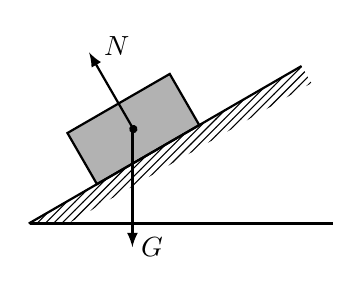
\begin{tikzpicture}[>=latex, thick,scale=1]
  % \useasboundingbox(-1,-0.75)rectangle(3.7,1.4);
  \draw [rotate=30, fill=black!30] (0,0) rectangle (1.5,.75);
  \fill [rotate=30, pattern = north east lines] (-1,0)--++(-30:0.5)--(3,-0.25) -- (3,0)--cycle;
  \draw[rotate=30] (-1,0)--(3,0);
  \draw[rotate=30, ->](.75,.375)--(.75,1.5);
  \draw[->](0.7-.25,0.7)--(0.7-.25,.7-1.5) ;
  \node at (.25,1.75){$N$};
  \draw(-.85,-.5)--(3,-.5);
  \fill [rotate=30](.75,.75/2) circle[radius=1.5pt];
  %\draw[rotate=30, ->] (.75,.75/2)--(.75+1,.75/2);
  %\node at (1.5, 1.25) {$f$};
  \node at (0.7,.7-1.5) {$G$};
\end{tikzpicture}
\end{document}